
    \begin{frame}{Gaussian Processes}
        A \textbf{\alert{Gaussian process}} (GP) is a collection of random variables \( f(\cdot) \) such that any finite collection \( \mathbf f = \{f(\mathbf x_1), f(\mathbf x_2), \dots, f(\mathbf x_N) \} \) follows a Gaussian distribution
        \[
            \mathbf f = f(\mathbf X) = \Big(f(\mathbf x_1),\dots,f(\mathbf x_N)\Big) \sim \mathcal{N}\Big(m(\mathbf X), \kappa(\mathbf X, \mathbf X)\Big)\,.
        \]
        Gaussian processes place a \textbf{probability distribution over functions}.

        Usually, 
        \[
            m(\mathbf x) = 0\quad \text{and} \quad            \kappa(\mathbf x_1, \mathbf x_2) = \sigma^2 \exp \left(- \frac{\|\mathbf x_1 - \mathbf x_2 \|_2^2}{2l^2} \right)\,.
        \]

    \end{frame}
    \begin{frame}

        \textbf{Hypothesis: } The unknown function \(f\) is a (noisy) sample from a Gaussian process.

        \begin{figure}
            \centering
            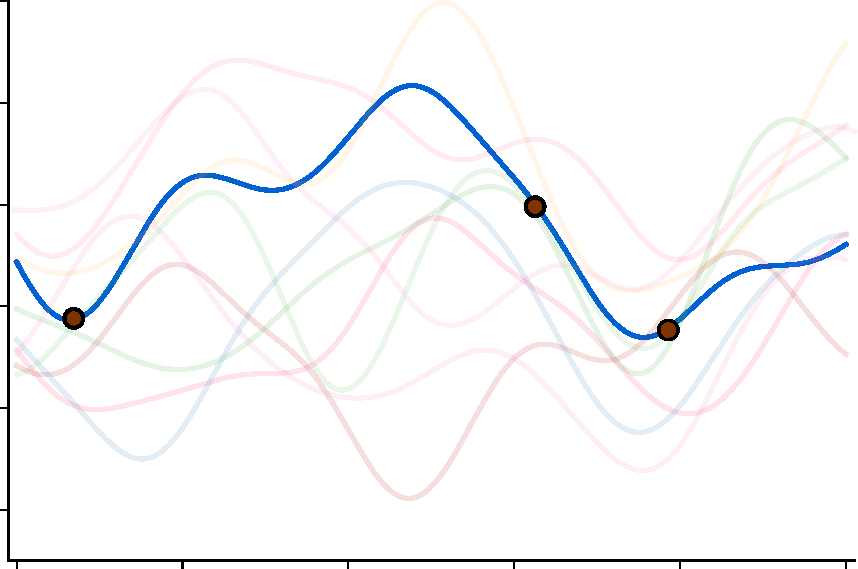
\includegraphics[width=0.7\textwidth]{imgs/GP_hypothesis.pdf}
        \end{figure}
    \end{frame}


    \begin{frame}
        For a regression problem, using,
        \begin{itemize}
            \item the Gaussian process prior over functions, \[ P(\mathbf f) = \mathcal{N}\Big(m(\mathbf X), \kappa(\mathbf X, \mathbf X)\Big)\,,\]
            \item a suitable likelihood  \[P(\mathbf y| \mathbf f) = \mathcal{N}(\mathbf f, \sigma^2 \mathbf I)\,.\]
        \end{itemize}
        Predictive distribution is computable in closed form
        \[
            P\big(f(\mathbf x^\star)|\mathbf y, \mathbf X\big) = \mathcal{N}( \mathbf \mu^\star, \mathbf \Sigma^\star)\,,
        \]
        with
        \begin{align*}
             \mathbf \mu^\star &= m(\mathbf x^\star) + \kappa(\mathbf x^\star, \mathbf X)(\kappa(\mathbf X, \mathbf X) + \sigma^2\mathbf I)^{-1}(\mathbf y - m(\mathbf X))\,,\\
             \mathbf \Sigma^\star &= \kappa(\mathbf x^\star, \mathbf x^\star) - \kappa(\mathbf x^\star, \mathbf X)(\kappa(\mathbf X, \mathbf X) + \sigma^2\mathbf I)^{-1}\kappa(\mathbf X, \mathbf x^\star)\,.
        \end{align*}
    \end{frame}

    \begin{frame}
            \begin{align*}
             \mathbf \mu^\star &= m(\mathbf x^\star) + \kappa(\mathbf x^\star, \mathbf X)(\kappa(\mathbf X, \mathbf X) + \sigma^2\mathbf I)^{-1}(\mathbf y - m(\mathbf X))\,,\\
             \mathbf \Sigma^\star &= \kappa(\mathbf x^\star, \mathbf x^\star) - \kappa(\mathbf x^\star, \mathbf X)(\kappa(\mathbf X, \mathbf X) + \sigma^2\mathbf I)^{-1}\kappa(\mathbf X, \mathbf x^\star)\,.
        \end{align*}
        \begin{figure}
            \centering
            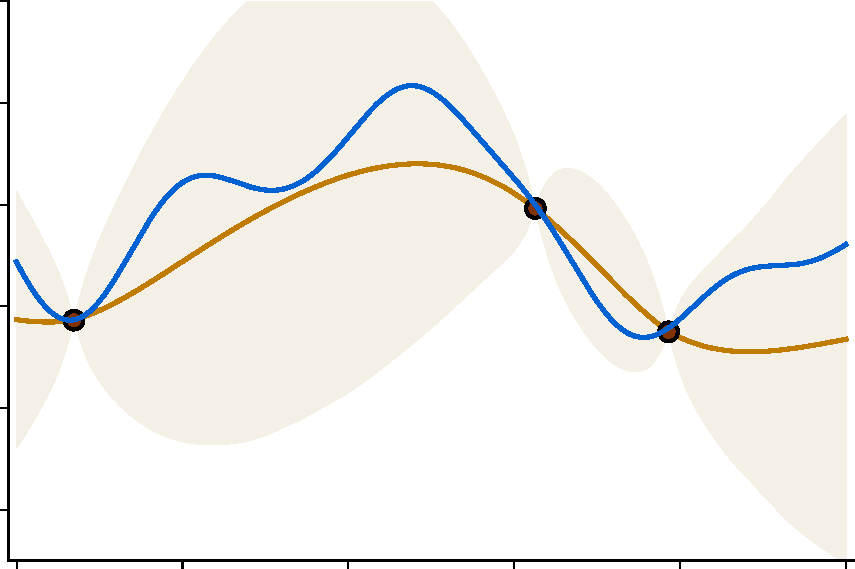
\includegraphics[width=0.75\textwidth]{imgs/GP_pred.pdf}
        \end{figure}
    \end{frame}

    \begin{frame}
        
        Hyper-parameters (kernel and likelihood) can be \textbf{optimized} using the marginal log likelihood:
        \[
            \log P(\mathbf y) = -\frac{1}{2}\mathbf y^T(\mathbf K + \sigma^2 \mathbf I)^{-1}\mathbf y - \frac{1}{2}\log \det (\mathbf K + \sigma^2 \mathbf I) - \frac{N}{2}\log 2\pi\,,
        \]
        with \(\mathbf K = \kappa(\mathbf X, \mathbf X)\).
        
        \vspace{1cm}
        
        \onslide<2->
        \textbf{\alert{Limitation.}} Requires the computation of \((\mathbf K + \sigma^2 \mathbf I)^{-1}\) which is \(\mathcal O(N^3)\).\\
        \textbf{\alert{Limitation.}} Mini-batches cannot be used for optimization.
    \end{frame}

    \subsection{Sparse Gaussian Processes}
    \begin{frame}{Sparse Gaussian Processes}
        \only<1>{
            Initialize a set of \textbf{\alert{inducing locations}}  \(\mathbf Z\) with \(|\mathbf Z| < |\mathbf X|\). For example \(\mathbf Z\) can be the centers of applying KMeans to \(\mathbf X\).
        }
        \only<2>{
            Set a variational distribution over the \textbf{\alert{inducing points}} \( \bm u = f(\mathbf Z)\), typically, \(Q(\bm u) = \mathcal{N}(\bm m, \bm S)\).
        }
        \only<3>{
            The approximated posterior predictive distribution is,
            \[
             Q( f(\mathbf x_\star)) = \int_{\bm u} P( f(\mathbf x_\star)| \bm u)Q(\bm u) = \mathcal{N}(\bm \mu, \bm \Sigma)
            \]
            is Gaussian and suitable for making predictions.
        }
            \begin{center}
                \includegraphics<1>[width=.7\linewidth]{imgs/GP_inducing_1.pdf}
                \includegraphics<2>[width=.7\linewidth]{imgs/GP_inducing_2.pdf}
                \includegraphics<3>[width=.6\linewidth]{imgs/GP_inducing_3.pdf}
            \end{center}
    \end{frame}
    \begin{frame}
            Minimize the ELBO to optimize \(Q(\bm u, \mathbf f)\), with \(\mathbf f = (f(\mathbf x_1),  \dots, f(\mathbf x_N))\),
            \begin{align*}
                Q^\star(\bm u,  \mathbf f) &= \argmin_{Q \in \mathcal{Q}}\, KL\Big(Q(\bm u,  \mathbf f)  \mid P(\bm u,  \mathbf f | \mathbf X, \mathbf y)\Big)\\
                &= \argmax_{Q \in \mathcal{Q}} \,\mathbb{E}_{Q( \mathbf f)}\Big[ \log P(\mathbf y | \mathbf X,  \mathbf f) \Big] - KL\Big(Q(\bm u) \mid P(\bm u) \Big)\,.\\
            \end{align*}    
            where 
            \begin{enumerate}
                \item \(P(\bm u)\) is given by the Gaussian Process distribution evaluated at \(\mathbf Z\).
                \item The Kullback-Leibler divergence is between Gaussian distributions.
                \item The data-fitting term can be computed for Gaussian likelihoods or approximated by quadrature.
            \end{enumerate}
    \end{frame}